\documentclass[../notes.tex]{subfiles}

\pagestyle{main}
\renewcommand{\chaptermark}[1]{\markboth{\chaptername\ \thechapter\ (#1)}{}}
\renewcommand{\thechapter}{\Roman{chapter}}
\setcounter{chapter}{6}

\begin{document}




\chapter{Band Theory in Solids}
\section{Module 21: Electronic Structure of Solids (1D Solids)}
\begin{itemize}
    \item \marginnote{2/5:}Solid silicon's symmetry space group would be $Fd\overline{3}m$.
    \item Suggested reading: \textcite{bib:bandTheory}.
    \begin{itemize}
        \item A rare less mathematical article on band theory that has taught generations of chemists; comes at it from a physics perspective.
    \end{itemize}
    \item To consider solids, let's first consider an infinite chain of hydrogen atoms.
    \begin{itemize}
        \item This should separate into \ce{H2} molecules (\textbf{Peierl's instability}); considering it to exist is a consequence of looking at chemistry through a physics perspective, where this is a simple model.
        \item However, other substances can have chains of $p_z$ orbitals, such as platinum atoms.
    \end{itemize}
    \item An imaginary zoo of hydrogen molecules (we use the limit of a cycle of hydrogen atoms to approximate an infinitely long chain):
    \begin{itemize}
        \item \ce{H2} has a bonding and antibonding MO.
        \item Cyclic \ce{H3+} is the most abundant ion in the universe (recently discovered by UChicago). One bonding and two antibonding orbitals.
        \item We can keep adding hydrogen atoms to our rings.
        \item For an infinitely long cycle of hydrogen atoms, we will have an infinite number of states close together that resembles a band in solids.
    \end{itemize}
    \item Back to the chain of \ce{H} atoms:
    \begin{itemize}
        \item The basis function on each lattice point is a \ce{H_{$1s$}} orbital; there are countably many.
        \item The appropriate SALCs $\psi_k$ are based in translating every orbital by a finite number of units:
        \begin{equation*}
            \psi_k = \sum_n\e[ikna]\phi_n
        \end{equation*}
        \begin{itemize}
            \item $a$ is the distance between neighboring hydrogen atoms.
            \item Since there are infinitely many translations, there should be infinitely many translational symmetry elements, so infinitely many irreducible representations, too.
            \item The coefficients $\e[ikna]$ come from \textbf{Bloch's theorem}.
        \end{itemize}
        \item In this formalism, $k$ is an index labeling irreducible representations of the translation group. $\psi$ transforms just like $a$, $e_1$, and $e_2$ (e.g., in the $C_5$ point symmetry group).
        \item This process of symmetry adaptation is called "forming Bloch functions."
    \end{itemize}
    \item Elementary band theory for extended solids:
    \begin{itemize}
        \item Energy bands in solids arise from overlapping atomic orbitals, which become the \textbf{crystal orbitals} that make up the bands.
        \item Recipe: Use LCAO (tight binding) approach.
        \item A crystal is a regular periodic array with translational symmetry.
        \item Periodic boundary conditions require $\psi(x+Na)=\psi(x)$, i.e., each wavefunction must be symmetry equivalent to the one in the neighboring cells.
        \item For a 1D solid with lattice constant $a$ and atom index $n$, Bloch's theorem tells us that the above SALC $\psi_k$ is a solution to the Schr\"{o}dinger equation.
    \end{itemize}
    \item If we calculate $\psi_0$ and $\psi_{\pi/a}$, we get the most and least bonding states possible, respectively (the least bonding state is the most antibonding state and has the highest energy).
    \begin{figure}[h!]
        \centering
        \begin{subfigure}[b]{0.35\linewidth}
            \centering
            \begin{tikzpicture}
                \draw (-2,0) -- (2,0);
                \foreach \x in {-1.5,-0.5,0.5,1.5} {
                    \filldraw [semithick,draw,fill=grt] (\x,0) circle (2.5mm);
                }
            \end{tikzpicture}
            \caption{$k=0$.}
            \label{fig:bandBonding-sa}
        \end{subfigure}
        \begin{subfigure}[b]{0.35\linewidth}
            \centering
            \begin{tikzpicture}
                \draw (-2,0) -- (2,0);
                \foreach \x in {-1.5,0.5} {
                    \filldraw [semithick,draw,fill=grt] (\x,0) circle (2.5mm);
                    \filldraw [semithick,draw,fill=white] ({\x+1},0) circle (2.5mm);
                }
            \end{tikzpicture}
            \caption{$k=\frac{\pi}{a}$.}
            \label{fig:bandBonding-sb}
        \end{subfigure}
        \caption{$s$ orbital bonding states.}
        \label{fig:bandBonding-s}
    \end{figure}
    \begin{align*}
        \psi_0 &= \phi_0+\phi_1+\phi_2+\phi_3+\cdots\\
        \psi_{\pi/a} &= \phi_0-\phi_1+\phi_2-\phi_3+\cdots
    \end{align*}
    \item At this point, we can construct a band between these two states.
    \begin{itemize}
        \item The band is \emph{almost} infinite; it's on the order of Avogadro's number.
        \item We have as many $k$ values as translations in the crystal or as many unit cells in a crystal.
    \end{itemize}
    \item \textbf{First Brillouin zone}: The region that covers all possible energy states that the crystal can have.
    \begin{itemize}
        \item It is $-\frac{\pi}{a}<k<\frac{\pi}{a}$; which is the range of all possible values that the sine function will give.
    \end{itemize}
    \item There is one energy level for each value of $k$, but $E(k)=E(-k)$.
    \item $k$ is proportional to the electron momentum, or electron velocity.
    \item Calculation of 1D band structure:
    \begin{itemize}
        \item We have $N$ atoms such that $\psi_k=\sum_{n=0}^N\e[inka]\phi_n$.
        \item The crystal Schr\"{o}dinger equation is $\hat{H}\Psi(k)=E(k)\Psi(k)$.
        \item Thus, the electron energies are given by
        \begin{equation*}
            E(k) = \frac{\ev{\hat{H}}{\psi}}{\braket{\psi}}
        \end{equation*}
        \item Recall that in Dirac's bra-ket notation, $\ev{\hat{H}}{\psi}\equiv\int\psi^*\hat{H}\psi\dd{\tau}$; for normalized atomic orbitals and ignoring overlap integrals:
        \begin{equation*}
            \braket{\phi_m}{\phi_n} =
            \begin{cases}
                1 & m=n\\
                0 & m\neq n
            \end{cases}
        \end{equation*}
        \item Also recall that
        \begin{equation*}
            \braket{\psi} = \sum_{m,n}\e[i(n-m)ka]\braket{\phi_m}{\phi_n} = N
        \end{equation*}
        \item Thus, we can calculate for on-site ($m=n$):
        \begin{equation*}
            \ev{\hat{H}}{\psi(k)} = \sum_n\ev{\hat{H}}{\phi_n} = N\alpha
        \end{equation*}
        And for resonance ($m\neq n$), where we need only consider the two nearest neighbors:
        \begin{equation*}
            \mel{\e[-inka]\phi_n}{\hat{H}}{\e[i(n\pm 1)ka]\phi_{n\pm 1}} = \beta\e[\pm ika]
        \end{equation*}
        \item Putting everything together, we have
        \begin{equation*}
            E(k) = \frac{\ev{\hat{H}}{\psi}}{\braket{\psi}} = \frac{N\alpha+N\beta(\e[ika]+\e[-ika])}{N} = \alpha+2\beta\cos(ka)
        \end{equation*}
    \end{itemize}
    \item \textbf{Zone center}: The state where all atomic orbitals are in phase (all bonding $\sigma$). \emph{Also known as} $\bm{\Gamma}$.
    \item \textbf{Zone border}: The state where all atomic orbitals are out of phase (all antibonding $\sigma^*$). \emph{Also known as} $\bm{X}$.
    \item Large numbers of MOs form bands of states.
    \item \textbf{Band structure}: The plot of $E$ as a function of $k$.
    \begin{itemize}
        \item The one we've derived so far is an s-shape curve.
    \end{itemize}
    \item The $p$-orbitals are opposite --- they form a bonding state with inverted phases.
    \begin{figure}[h!]
        \centering
        \begin{subfigure}[b]{0.35\linewidth}
            \centering
            \begin{tikzpicture}
                \foreach \x in {-1,0,1} {
                    \draw [densely dashed] (\x,-0.3) -- ++(0,0.6);
                }
                \foreach \x in {-1.5,-0.5,0.5,1.5} {
                    \filldraw [semithick,draw,fill=grt] (\x,0)
                        to [out=90,in=90,out looseness=0.5] ({\x+0.4},0)
                        to [out=-90,in=-90,in looseness=0.5] cycle
                    ;
                    \draw [semithick] (\x,0)
                        to [out=90,in=90,out looseness=0.5] ({\x-0.4},0)
                        to [out=-90,in=-90,in looseness=0.5] cycle
                    ;
                }
            \end{tikzpicture}
            \caption{$k=0$.}
            \label{fig:bandBonding-pa}
        \end{subfigure}
        \begin{subfigure}[b]{0.35\linewidth}
            \centering
            \begin{tikzpicture}
                \path (0,-0.3) -- ++(0,0.6);
                \foreach \x in {-1.5,0.5} {
                    \filldraw [semithick,draw,fill=grt] (\x,0)
                        to [out=90,in=90,out looseness=0.5] ({\x+0.4},0)
                        to [out=-90,in=-90,in looseness=0.5] cycle
                    ;
                    \draw [semithick] (\x,0)
                        to [out=90,in=90,out looseness=0.5] ({\x-0.4},0)
                        to [out=-90,in=-90,in looseness=0.5] cycle
                    ;
                }
                \foreach \x in {-0.5,1.5} {
                    \draw [semithick] (\x,0)
                        to [out=90,in=90,out looseness=0.5] ({\x+0.4},0)
                        to [out=-90,in=-90,in looseness=0.5] cycle
                    ;
                    \filldraw [semithick,draw,fill=grt] (\x,0)
                        to [out=90,in=90,out looseness=0.5] ({\x-0.4},0)
                        to [out=-90,in=-90,in looseness=0.5] cycle
                    ;
                }
            \end{tikzpicture}
            \caption{$k=\frac{\pi}{a}$.}
            \label{fig:bandBonding-pb}
        \end{subfigure}
        \caption{$p$ orbital bonding states.}
        \label{fig:bandBonding-p}
    \end{figure}
    \item The analysis of Figures \ref{fig:bandBonding-s} and \ref{fig:bandBonding-p} can be done for many more types of orbitals, including $p_z$, $d_{z^2}$, and $d_{xz}$.
    \item Bonding orbital bands run uphill (concave upwards $E(k)$) at $k=0$ and antibonding orbital bands run downhill (concave downwards $E(k)$) at $k=0$.
    \item Energy bands run from $\alpha+2\beta$ to $\alpha-2\beta$ since $\beta$ is negative for $s$ orbitals.
    \item \textbf{Density of states}: The number of energy levels in the energy interval $\Delta E$. \emph{Also known as} \textbf{DOS}.
    \begin{figure}[h!]
        \centering
        \begin{tikzpicture}
            \footnotesize
            \begin{scope}[xshift=-4.85cm]
                \foreach \y in {0.4,0.5,...,3} {
                    \draw [ultra thick] (0,\y) -- ++(0.5,0);
                }
                \node at (1.15,1.7) {$\equiv$};
            \end{scope}
            \begin{scope}[xshift=-3cm]
                \draw [thick] (0,0.4) rectangle (0.5,3);
                \node at (1.15,1.7) {$\equiv$};
            \end{scope}
            \begin{scope}
                \draw (4,0) node[below]{$\pi/a$} -- node[below=2mm]{\small$k\longrightarrow$} (0,0) node[below]{$0$} -- node[left=2mm,align=center]{\small$\uparrow$\\$E$} (0,3.3);
                \draw (0.1,0.5) -- ++(-0.2,0) node[left]{$\alpha+2\beta$};
                \draw (0.1,2.9) -- ++(-0.2,0) node[left]{$\alpha-2\beta$};
    
                \draw [grx,thick] (0,0.5) cos (2,1.7) node[above left,black]{$E(k)$} sin (4,2.9);
            \end{scope}
            \begin{scope}[xshift=6cm]
                \draw (3,0) -- node[below=2mm]{\small$\text{DOS}\longrightarrow$} (0,0) node[below]{$0$} -- node[left=2mm,align=center]{\small$\uparrow$\\$E$} (0,3.3);
    
                \draw [gry,thick,rotate=90] (0.5,0) -- (0.5,-2) sin (1.7,-0.5) cos (2.9,-2) -- (2.9,0);
            \end{scope}
        \end{tikzpicture}
        \caption{Density of states.}
        \label{fig:densityOfStates}
    \end{figure}
    \begin{itemize}
        \item Proportional to the inverse slope of the band; steep bands with large overlap yield a small DOS, and vice versa for flat bands.
        \item Reality check: PES for a long-chain alkane (\ce{C36H74}) shows this inverse DOS relationship for a little while.
    \end{itemize}
\end{itemize}



\section{Module 22: Electronic Structure of Solids (2D and 3D solids)}
\begin{itemize}
    \item 2D band structure:
    \begin{itemize}
        \item Simple H\"{u}ckel: A two-dimensional square net ($s$ orbitals only (or $p_z$)).
        \begin{equation*}
            \psi(k) = \sum_{m,n}\e[ik_xma+ik_yna]\cdot\phi_{m,n}
        \end{equation*}
        \item Consider the \textbf{crystal orbitals} at special $k$ points (high symmetry).
        \item The \textbf{Brillouin zone} is 2D here (we have a \textbf{wave vector}).
        \begin{figure}[h!]
            \centering
            \begin{tikzpicture}[
                every node/.append style={black}
            ]
                \footnotesize
                \path (-2,0) -- (2,0);
                \draw (-1,-1) rectangle (1,1);

                \draw [gry,thick,-stealth] (0,0) -- (1.5,0) node[right]{$\vec{b}_1$};
                \draw [gry,thick,-stealth] (0,0) -- (0,1.5) node[above]{$\vec{b}_2$};

                \fill [grx] (0,0) circle (2pt) node[below left]{$\Gamma$};
                \fill [grx] (0,1) circle (2pt) node[above left]{$X$};
                \fill [grx] (1,1) circle (2pt) node[above right]{$M$};
                \fill [grx] (1,0) circle (2pt) node[above right]{$X$};
            \end{tikzpicture}
            \caption{2D Brillouin zone.}
            \label{fig:brillouinZone-2D}
        \end{figure}
        \begin{figure}[h!]
            \centering
            \begin{subfigure}[b]{0.24\linewidth}
                \centering
                \begin{tikzpicture}[scale=0.8]
                    \draw (0,0) grid (3,3);
                    \foreach \x in {0,...,3} {
                        \foreach \y in {0,...,3} {
                            \filldraw [semithick,draw,fill=grt] (\x,\y) circle (3.125mm);
                        }
                    }
                \end{tikzpicture}
                \caption{$\Gamma$: $k_x,k_y=0$.}
                \label{fig:specialKPointsa}
            \end{subfigure}
            \begin{subfigure}[b]{0.24\linewidth}
                \centering
                \begin{tikzpicture}[scale=0.8]
                    \draw (0,0) grid (3,3);
                    \foreach \x in {0,2} {
                        \foreach \y in {0,...,3} {
                            \filldraw [semithick,draw,fill=grt] (\x,\y) circle (3.125mm);
                        }
                    }
                    \foreach \x in {1,3} {
                        \foreach \y in {0,...,3} {
                            \filldraw [semithick,draw,fill=white] (\x,\y) circle (3.125mm);
                        }
                    }
                \end{tikzpicture}
                \caption{$X$: $k_x=\pi/a,k_y=0$.}
                \label{fig:specialKPointsb}
            \end{subfigure}
            \begin{subfigure}[b]{0.24\linewidth}
                \centering
                \begin{tikzpicture}[scale=0.8]
                    \draw (0,0) grid (3,3);
                    \foreach \x in {0,2} {
                        \foreach \y in {1,3} {
                            \filldraw [semithick,draw,fill=grt] (\x,\y) circle (3.125mm);
                        }
                        \foreach \y in {0,2} {
                            \filldraw [semithick,draw,fill=grt] ({\x+1},\y) circle (3.125mm);
                        }
                    }
                    \foreach \x in {0,2} {
                        \foreach \y in {0,2} {
                            \filldraw [semithick,draw,fill=white] (\x,\y) circle (3.125mm);
                        }
                        \foreach \y in {1,3} {
                            \filldraw [semithick,draw,fill=white] ({\x+1},\y) circle (3.125mm);
                        }
                    }
                \end{tikzpicture}
                \caption{$M$: $k_x,k_y=\pi/a$.}
                \label{fig:specialKPointsc}
            \end{subfigure}
            \begin{subfigure}[b]{0.24\linewidth}
                \centering
                \begin{tikzpicture}[scale=0.8]
                    \draw (0,0) grid (3,3);
                    \foreach \x in {0,...,3} {
                        \foreach \y in {1,3} {
                            \filldraw [semithick,draw,fill=grt] (\x,\y) circle (3.125mm);
                        }
                    }
                    \foreach \x in {0,...,3} {
                        \foreach \y in {0,2} {
                            \filldraw [semithick,draw,fill=white] (\x,\y) circle (3.125mm);
                        }
                    }
                \end{tikzpicture}
                \caption{$X$: $k_x=0,k_y=\pi/a$.}
                \label{fig:specialKPointsd}
            \end{subfigure}
            \caption{Special $k$ points.}
            \label{fig:specialKPoints}
        \end{figure}
        \begin{itemize}
            \item The center is the $\Gamma$ point ($k_x=k_y=0$; every orbital is surrounded by 4 orbitals of matching phase). The midpoint of the lines are called $X$ points ($k_x=\frac{\pi}{a},k_y=0$, and vice versa; every orbital is surrounded by 2 orbitals of matching phase and 2 orbitals of unlike phase). The maximum point is the $M$ point ($k_x=k_y=\frac{\pi}{a}$; every orbital is surrounded by 4 orbitals of unlike phase).
        \end{itemize}
        \item Calculating $E(k)$ in two dimensions.
        \begin{equation*}
            E(k) = \alpha+2\beta(\cos(k_xa)+\cos(k_ya))
        \end{equation*}
        \begin{figure}[H]
            \centering
            \begin{tikzpicture}[scale=0.9]
                \footnotesize
                \draw (3.41,0) -- node[below=3mm]{\small$k\longrightarrow$} (0,0) node[below]{$\Gamma$} -- node[left=1mm,align=center]{\small$\uparrow$\\$E$} (0,6);
                \draw [densely dashed,|-] (1,6) -- ++(0,-6) node[below]{$X$};
                \draw [densely dashed,|-] (2,6) -- ++(0,-6) node[below]{$M$};
                \draw [densely dashed,|-] (3.41,6) -- ++(0,-6) node[below]{$\Gamma$};

                \draw [grx,thick] (0,1.5) cos (0.5,2.5) sin (1,3.5) cos (1.5,4.5) sin (2,5.5) cos (2.71,3.5) sin (3.41,1.5);
            \end{tikzpicture}
            \caption{Schematic band structure (2D).}
            \label{fig:schematicBands-2D}
        \end{figure}
        \item Our schematic band structure (Figure \ref{fig:schematicBands-2D}) traces values along a 1D path in two-space from $\Gamma\to X\to M\to\Gamma$.
    \end{itemize}
    \item \marginnote{2/8:}The bandwidth $4|\beta|$ is proportional to the degree of interaction between neighboring orbitals.
    \begin{itemize}
        \item Since $\beta$ is the interaction integral and $E(k)$ varies from $\alpha-2\beta$ to $\alpha+2\beta$.
    \end{itemize}
    \item For $p_\sigma$ orbitals, $\beta>0$.
    \item Deriving the density of states formula:
    \begin{itemize}
        \item We often simplify $E(k)$ with the first term of the Taylor series expansion; this gives us
        \begin{equation*}
            E = \frac{\hbar}{2m}k^2
        \end{equation*}
        \item This implies that $E\propto k^2$ and, hence, $k\propto\sqrt{E}$.
        \item Thus, the one-dimensional density $D_{1d}(k)$ of states as a function of $k$ is $\dv*{N(k)}{k}=1$ since the number of states is evenly distributed along the $k$ axis (i.e., in Figure \ref{fig:densityOfStates}).
        \item It follows that the one-dimensional density $D_{1d}(E)$ of states as a function of $E$ is
        \begin{equation*}
            D_{1d}(E) = \dv{N(E)}{E}
            = \dv{N(k)}{k}\dv{k}{E}
            \propto 1\cdot\frac{1}{\sqrt{E}}
            = \frac{1}{\sqrt{E}}
        \end{equation*}
    \end{itemize}
    \item For each orbital, there is a unique path akin to Figure \ref{fig:schematicBands-2D}. The combination of all of these \textbf{bands} in one graph characterizes a material.
    \item \textbf{Wigner-Seitz cell} (of the reciprocal lattice): The first Brillouin zone, or FBZ.
    \begin{itemize}
        \item A primitive cell with a lattice point at its center.
        \item A 3D discrete Fourier transform of the lattice.
        \item Has $k_{x,y,z}$.
        \item What is "d.I." and "r.I."?
        \item We once again can find high symmetry points and directions akin to those in Figure \ref{fig:brillouinZone-2D}.
    \end{itemize}
    \begin{figure}[h!]
        \centering
        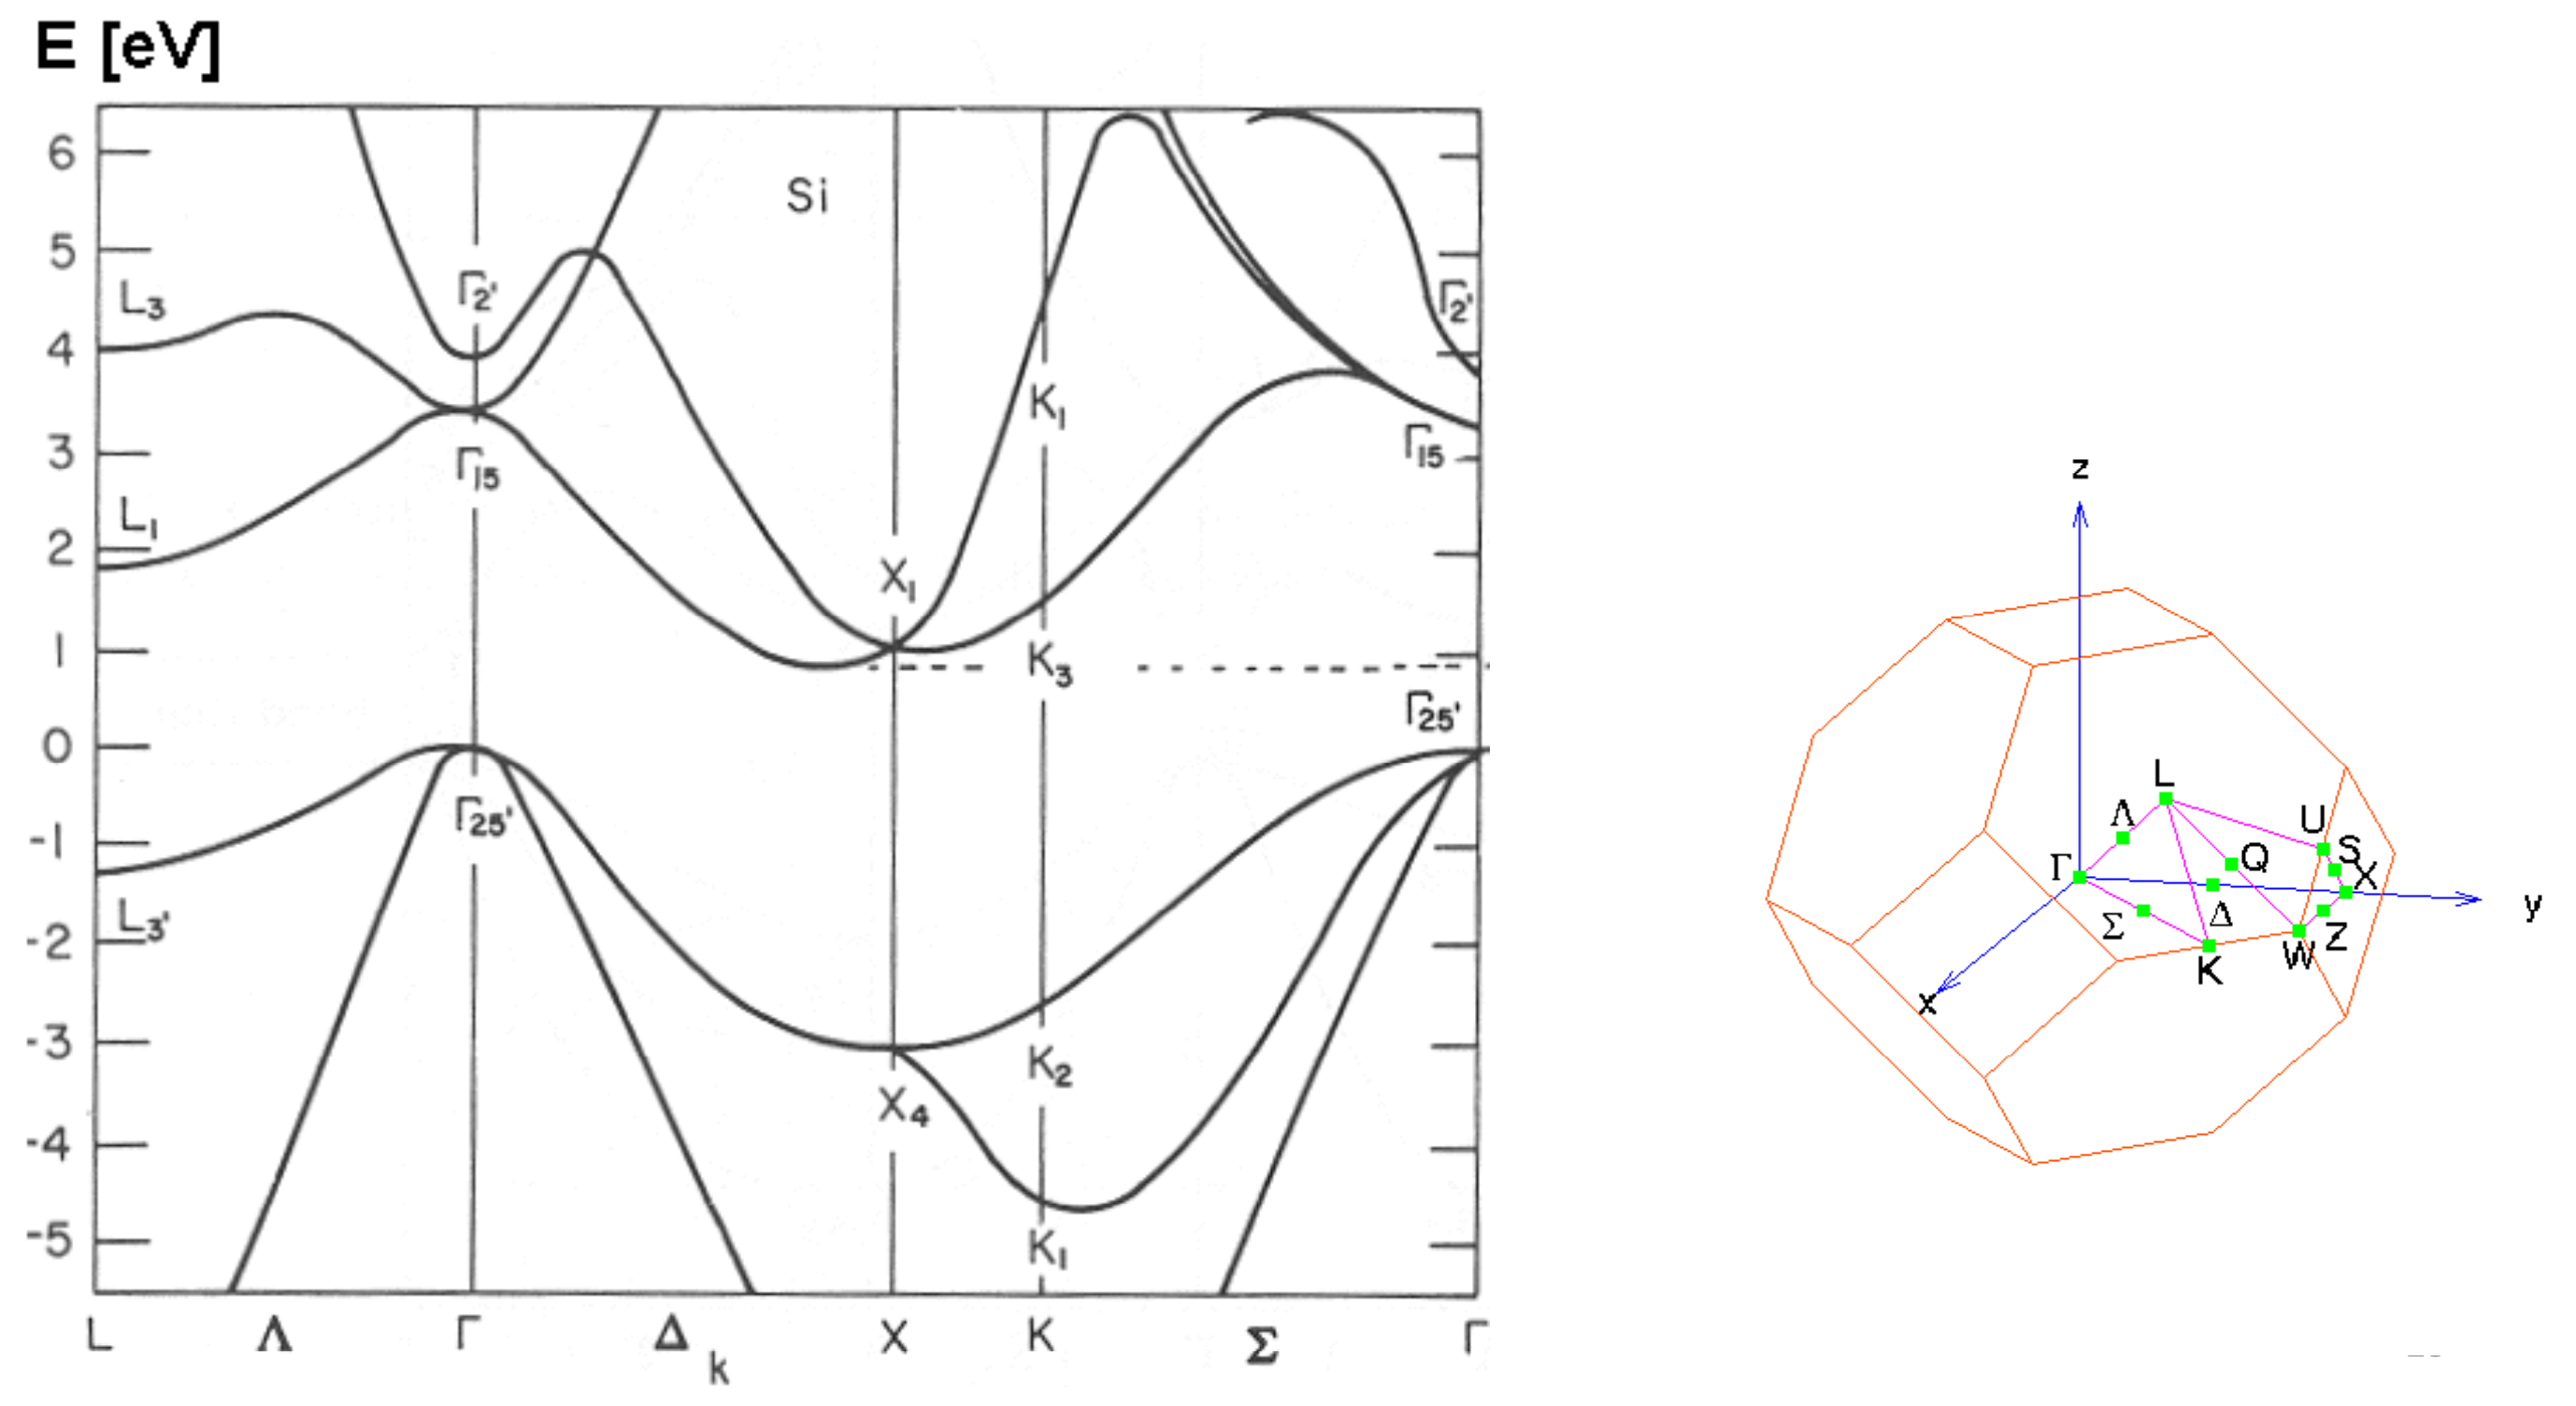
\includegraphics[width=0.75\linewidth]{../ExtFiles/bandStructure-Si.png}
        \caption{Electronic band structure of \ce{Si}.}
        \label{fig:bandStructure-Si}
    \end{figure}
    \item Electronic band structure is calculated within the first Brilluoin zone to give us the electronic band structure of a solid.
    \item \textbf{Angle-resolved photoemission spectroscopy}\footnote{Figure 7.20 in \textcite{bib:APChemNotes} actually refers to this kind of photoelectron spectroscopy!}: If the incoming photon's energy is greater than the electron's ginding energy, the electron will eventually be emitted with a characteristic kinetic energy and angle relative to the surface normal. This angle is related to the electron's crystal momentum. The Bloch wave vector is linked to the measured electron's momentum. \emph{Also known as} \textbf{ARPES}.
    \begin{itemize}
        \item Indeed, ARPES can be used to reconstruct the band structure of a solid. The bands are real!
    \end{itemize}
\end{itemize}



\section{Module 23: Filling Bands With Electrons}
\begin{itemize}
    \item The Fermi-Dirac statistics and Fermi Energy:
    \begin{itemize}
        \item At $T=0$, we expect all of the atoms in a solid to be in the ground state. The distribution of electrons (fermions) at the various energy levels is governed by the Fermi-Dirac distribution:
        \begin{equation*}
            F(E) = \frac{1}{1+\exp\left( \frac{E-E_F}{kT} \right)}
        \end{equation*}
        where $E_F$ is the Fermi energy.
        \begin{itemize}
            \item $F(E)$ is the probability to fill the states with a given energy $E$.
        \end{itemize}
        \item When $T=\SI{0}{\kelvin}$, the Fermi energy is the energy of the last occupied state. Moreover, 
        \item The Fermi energy is the energy of the last occupied state at $T=\SI{0}{\kelvin}$; it is proportional to the square of the Fermi state $k_F$, i.e., $E_F\propto k_F^2$.
    \end{itemize}
    \item If $T>0$, then:
    \begin{itemize}
        \item We fill the states from bottom to top.
        \item Instead of having a sharp shift from occupied to unoccupied states, we have a sort-of washed-out step function.
        \item Far below $E_F$, $F(E)=1$; far above $E_F$, $F(E)=0$. In the small \textbf{Fermi window} (aka. \textbf{Fermi level}) at the border (where the washed-out step function is), $0<F(E)<1$.
        \begin{itemize}
            \item The Fermi window is $4kbt$.
        \end{itemize}
        \item It is in the Fermi level that all of the important stuff happens (i.e., electrons flowing in metals).
    \end{itemize}
    \item If the gap (range where $\text{DOS}(E)=0$) in the density of states at the Fermi level is smaller than $\SI{3}{eV}$, then we have a semiconductor. If larger, we have an insulator. If 0, we have a conductor. Magnitude of DOS at Fermi level correlates with conductivity (e.g., \ce{Al} has a higher DOS at the Fermi level than \ce{Ag}, and we observe that \ce{Al} is more conductive than \ce{Ag}).
    \begin{itemize}
        \item In metals and insulators, the Fermi level is within bands.
        \item In semiconductors, it is between bands.
        \item In physics, everything is a metal or insulator; semiconductors are a constructed perspective.
    \end{itemize}
    \item Fermi sphere:
    \begin{itemize}
        \item The surface of the Fermi sphere separates occupied and unoccupied states in $k$-space.
        \item Bounded by Fermi surface.
        \item Radius is Fermi wave vector $k_F=\sqrt[3]{3\pi^2n}$ where $n$ is a parameter related to the density of electrons.
        \item Fermi energy: $E_F=\hbar^2k_F^2/2m$.
        \item Fermi momentum: $p_F=\hbar k_F$.
        \item Fermi velocity: $v_F=\hbar k_F/m$.
        \item Fermi temperature: $T_F=E_F/k_B$.
    \end{itemize}
    \item Electrons at $T=\SI{0}{\kelvin}$ still move very quickly (approximately $0.06$ the speed of light) since they're quantum particles (not classical ones).
    \item 3D density of states:
    \begin{itemize}
        \item The density of states $g(E)$ is the number of one-electron states (including spin multiplicity) per unit energy and volume:
        \begin{equation*}
            g(E)_{3D} \equiv \frac{1}{V}\dv{N}{E}
        \end{equation*}
        \begin{itemize}
            \item $N$ is twice the product of the Fermi sphere volume and the number of levels per unit volume.
        \end{itemize}
        \item Thus,
        \begin{equation*}
            N = 2\times\frac{4}{3}\pi k^3\times\frac{V}{8\pi^3} = \frac{V}{3\pi^2\hbar^3}(2m^*E)^{3/2}
        \end{equation*}
        so
        \begin{equation*}
            g(E)_{3D} = \frac{1}{V}\dv{N}{E} = \frac{1}{2\pi^2}\left( \frac{2m^*}{\hbar^2} \right)^{3/2}\sqrt{E}
        \end{equation*}
        \item Take CHEM 39000 Solids, Materials, and Surfaces to learn more.
    \end{itemize}
\end{itemize}



\section{Hoffmann's Band Theory}
\emph{From \textcite{bib:bandTheory}.}
\begin{itemize}
    \item \marginnote{3/8:}Lists and attempts to resolve some minor problems at the intersection of solid-state chemistry and physics/the rest of chemistry.
    \item An understanding of the electromagnetic properties of solids hinges on an understanding of modern solid-state physics, or band theory.
    \begin{itemize}
        \item Yet while physicists can better \emph{describe} (i.e., mathematically) a solid-state system, chemists better \emph{understand} them (i.e., intuitively).
    \end{itemize}
    \item Solid state chemists must consider not just ionic packing and electrostatic properties, but covalency and other more "molecular" notions.
    \item \textbf{Zintl concept}: "In some compounds \ce{A_xB_y}, where \ce{A} is very electropositive relative to a main-group element \ce{B}, one could just think, that's all, think that the \ce{A} atoms transfer their electrons to the \ce{B} atoms, which they then use to form bonds" \parencite[847]{bib:bandTheory}.
    \item Three big problems (in Hoffmann's opinion; in some others' opinions, these may not be issues at all):
    \begin{enumerate}
        \item Some lack of knowledge (therefore fear) of solid-state physics language on the part of chemists.
        \item Insufficient appreciation of the chemists' intuitive feeling for bonding on the part of physicists.
        \item Not enough reaching out for connections with molecular chemistry on the part of solid-state chemists.
    \end{enumerate}
    \item This paper will largely focus on problem 1, taking a simple (indeed, oversimplified) approach that utilizes the extended H\"{u}ckel model or the \textbf{tight-binding method} (with overlap).
    \item \textbf{Tight-binding method} (with overlap): The solid-state analogue of the extended H\"{u}ckel model.
    \item \textbf{Peierls distortion}: The instability of the band for an equally spaced one-dimensional polymer of \ce{H} atoms. \emph{Also known as} \textbf{strong electron-phonon coupling}, \textbf{pairing distortion}, \textbf{$\bm{2k_F}$ instability}.
    \begin{itemize}
        \item This will lead to a one-dimensional \ce{H}-atom polymer to form a chain of hydrogen molecules at ambient pressure.
    \end{itemize}
    \item \textbf{Applying cyclic boundary conditions}: Thinking of a long chain as an imperceptibly bent segment of a large ring.
    \begin{figure}[h!]
        \centering
        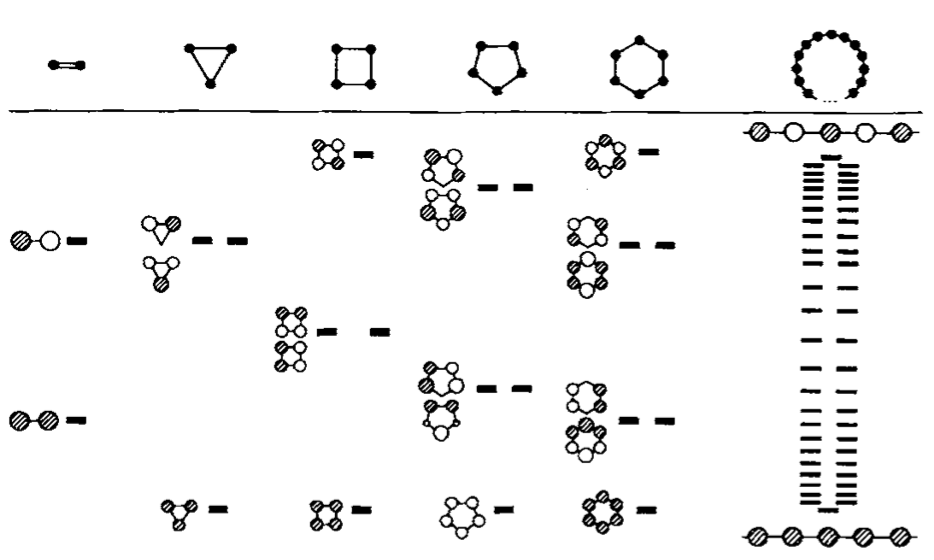
\includegraphics[width=0.5\linewidth]{../ExtFiles/zooOfHAtoms.png}
        \caption{Orbitals in \ce{H}-atom rings.}
        \label{fig:zooOfHAtoms}
    \end{figure}
    \begin{itemize}
        \item We apply cyclic boundary conditions to the 1D \ce{H}-atom chain.
    \end{itemize}
    \item In a cyclic structure, "except for the lowest (and occasionally the highest) level, the orbitals come in degenerate pairs" \parencite[848]{bib:bandTheory}.
    \begin{itemize}
        \item The number of nodes also increases as one rises in energy: The lowest level is nodeless, the highest has the maximum number of nodes, and a growing number of nodes are present in between.
    \end{itemize}
    \item Introduces Bloch's theorem.
    \item The larger the absolute value of $k$ (within the FBZ), the more nodes in the wave function.
    \item The number of values of $k$ is equal to the number of translations in the crystal, or the number of microscopic unit cells in the macroscopic crystal.
    \begin{itemize}
        \item And this will be on the order of Avogadro's number $N_A$.
        \item Keep in mind that although the $E(k)$ curve in Figure \ref{fig:densityOfStates} appears continuous, there are only a finite (albeit very large) number of points in $k$-space.
    \end{itemize}
    \item "There is an energy level for each value of $k$ (actually a degenerate pair of levels for each pair of positive and negative $k$ values)" \parencite[848]{bib:bandTheory}.
    \begin{itemize}
        \item Since $E(k)=E(-k)$ (as can be proved in an easy but unreferenced theorem), most graphical representations of the function depict $E(|k|)$ and label it $E(k)$.
    \end{itemize}
    \item \textbf{Reciprocal space}: The space of $k$, in which the allowed values of $k$ are equally spaced. \emph{Also known as} \textbf{momentum space}, \textbf{$\bm{k}$-space}.
    \begin{itemize}
        \item $k$ is related to momentum because $k=1/\lambda$, and from de Brogelie, $\lambda=h/p$.
        \item This means that $k$ is not only a symmetry label and a node counter, but also a wave vector (thus a measure of momentum).
    \end{itemize}
    \item \textbf{Band width}: The difference in energy between the highest and lowest levels of the band. \emph{Also known as} \textbf{dispersion}.
    \begin{itemize}
        \item Determined by the overlap between the interacting orbitals of neighboring unit cells.
    \end{itemize}
    \item Bands extend unsymmetrically around their origin (which is the energy of a free \ce{H} atom at $\SI{-13.6}{eV}$) because of the inclusion of overlap in calculations.
    \begin{itemize}
        \item Note that bands with greater band width are \emph{more} symmetric about the origin, i.e., as $4|\beta|$ increases in Figure \ref{fig:densityOfStates}, the $E(k)$ band centers itself more around the origin.
    \end{itemize}
    \item To recap band width and the import of bands running up or down, "band width is set by inter-unit-cell overlap, and the way bands run is determined by the topology of that overlap" \parencite[849]{bib:bandTheory}.
    \item Discusses stacking of platinum square-planar complexes, incorporating CFT and MO theory to build its band structure\footnote{If I have time to come back and digest this, it would be fascinating and educational.}.
    \item \textbf{Fermi level}: The HOMO of a solid.
    \begin{itemize}
        \item The alternate thermodynamic definition (appropriate to both metals and semiconductors) is what was discussed in lecture.
    \end{itemize}
    \item Determining the Fermi level of \ce{[PtH4]^2-}:
    \begin{figure}[H]
        \centering
        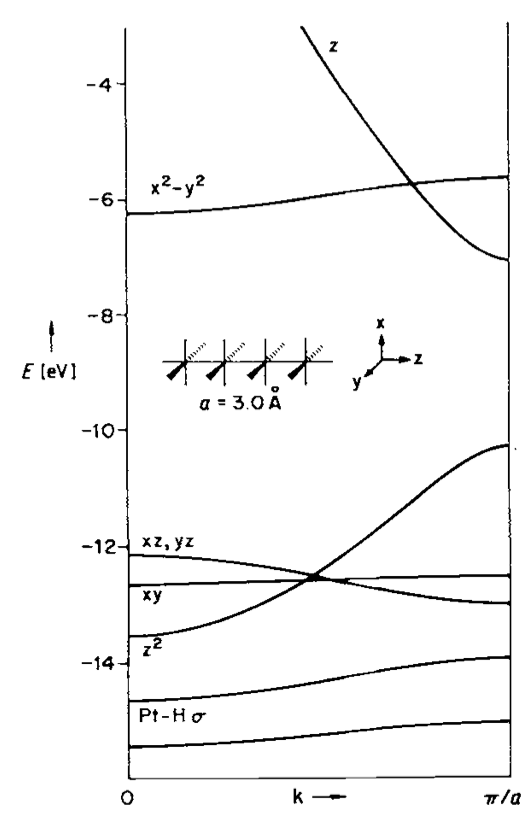
\includegraphics[width=0.3\linewidth]{../ExtFiles/bandStructure-PtH4.png}
        \caption{Electronic band structure of \ce{[PtH4]^2-}.}
        \label{fig:bandStructure-PtH4}
    \end{figure}
    \begin{itemize}
        \item Each platinum atom is $d^8$.
        \item From the band structure, the $\frac{8\text{ electrons}}{2\text{ electrons per level}}=4$ lowest energy bands are the $z^2$, $xy$, $xz$, and $yz$ bands (with the latter two degenerate).
        \item Thus, these will be completely filled, making the Fermi level the top of the band that protrudes the highest (the $z^2$ band).
    \end{itemize}
    \item Although this is not formal, we can tell from Figures \ref{fig:bandBonding-s} and \ref{fig:bandBonding-p} that the bottom of each band is bonding and the top, antibonding.
    \begin{itemize}
        \item Thus, filling a band entirely provides no net bonding (and, in fact, net antibonding).
    \end{itemize}
    \item Returning to our \ce{[PtH4]^2-} example:
    \begin{itemize}
        \item The stack likely forms due to a combination of van der Waals attractions and a combination of orbital interactions involving the mixing of the $d_{z^2}$ and $p_z$ bands.
        \item Additionally, \ce{Pt-Pt} separation likely decreases on oxidation because losing electrons takes them away from the higher energy antibonding portions of the bands, enhancing bonding character.
        \begin{itemize}
            \item A typical oxidation of 0.3 electrons per \ce{Pt} atom empties the top 15\% of the $d_{z^2}$ band, which had been strongly $\sigma^*$ antibonding.
        \end{itemize}
        \item Importantly, "the oxidized material\dots has its Fermi level in a band; i.e., there is a zero band gap between filled and empty levels. The unoxidized cyanoplatinates have a substantial gap --- they are semiconductors or insulators. The oxidized materials are good low dimensional conductors" \parencite[851-52]{bib:bandTheory}.
    \end{itemize}
    \item For good conductivity, the Fermi level must cut one or more bands. However, we must also beware of distortions which open up gaps at the Fermi level and exceedingly narrow bands that are cut by the Fermi level.
    \item Density of states resolves the following conundrum:
    \begin{itemize}
        \item In a discrete molecule, we can single out one or a few orbitals (HOMO, LUMO) as being the frontier orbitals responsible for geometry, reactivity, etc.
        \item There is no way that a few orbitals determine the properties of a solid.
        \item How, then, can we determine such properties?
        \item We can do so by looking at bunches of levels (all those in a given energy interval between $E$ and $E+\dd{E}$).
    \end{itemize}
    \item The shapes of DOS curves are predictable from the band structures.
    \item "The integral of DOS up to the Fermi level is the total number of occupied MOs. Multiplied by two, it's the total number of electrons" \parencite[852]{bib:bandTheory}.
    \begin{itemize}
        \item Thus, the DOS curves plot the distribution of electrons in energy.
    \end{itemize}
    \item DOS curves represent a return from reciprocal space to real space since it's an average over the Brillouin zone, i.e., over all $k$ that might give molecular orbitals at the specified energy.
    \begin{itemize}
        \item One benefit to this is that it facilitates intuitively sketching the DOS from the MO diagram using our knowledge of orbital interactions in space, as we did when rationalizing the \ce{[PtH4]^2-} band structure.
    \end{itemize}
    \item Continues into some higher level 1D topics, from which there are a couple of relevant points:
    \begin{itemize}
        \item "The Jahn-Teller theorem says that such a situation necessitates a large interaction of vibrational and electronic motion. It states that there must be at least one normal mode of vibration which will break the degeneracy and lower the energy of the system (and, of course, lower its symmetry). It even specifies which vibrations would accomplish this" \parencite[862]{bib:bandTheory}.
        \item The Peierls distortion is the solid-state counterpart of the Jahn-Teller distortion, a phenomenon where electrons in a partially filled band can distort the system (\'{a} la Jahn-Teller) to lower its energy and open up a gap at the Fermi level.
    \end{itemize}
    \item In higher dimensions, $\vec{k}$ must be treated as a vector with components in reciprocal space.
    \begin{figure}[h!]
        \centering
        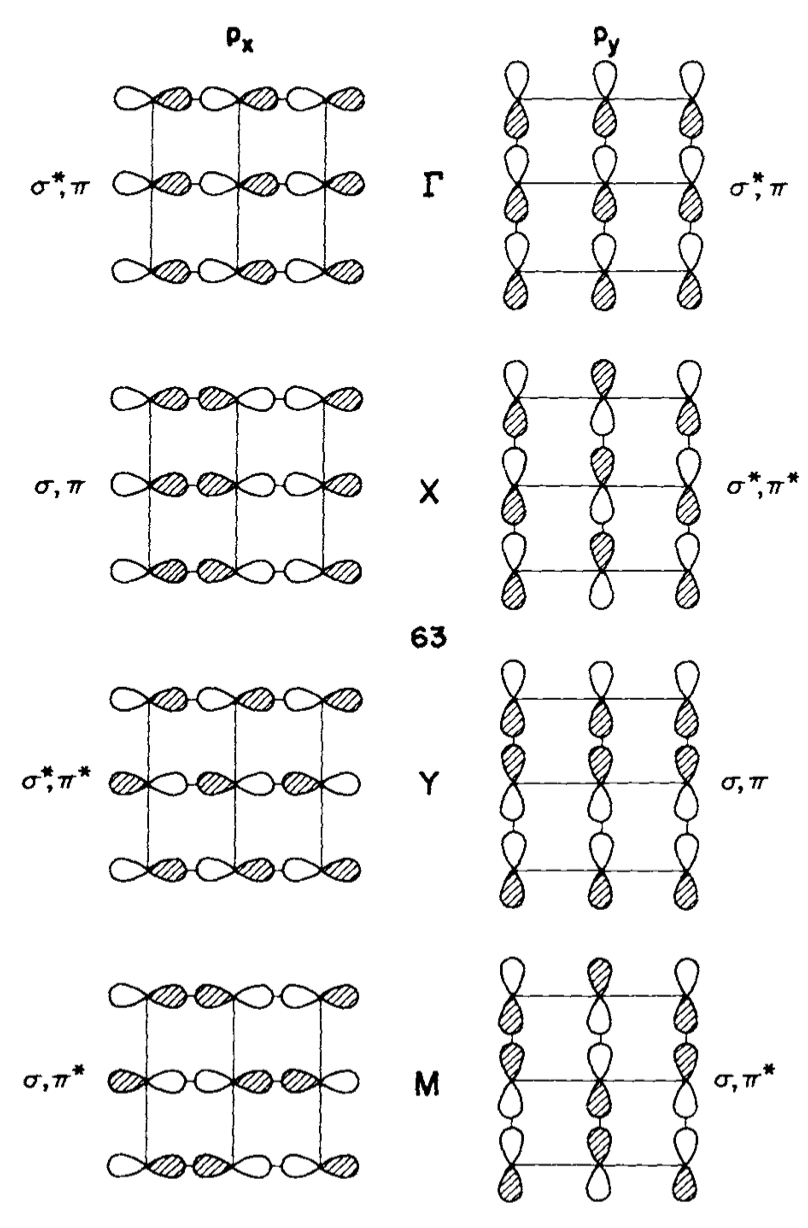
\includegraphics[width=0.45\linewidth]{../ExtFiles/bandBonding-pxpy2D.png}
        \caption{2D $p_{x,y}$ orbital bonding states.}
        \label{fig:bandBonding-pxpy2D}
    \end{figure}
    \item When we include $p$ orbitals in our 2D lattice, the $\Gamma$, $X$, and $M$ configurations have varying $\sigma$ / $\sigma^*$ character and $\pi$ / $\pi^*$ character (see Figure \ref{fig:bandBonding-pxpy2D}).
\end{itemize}




\end{document}